\chapter{Kalman Filters}
\label{Kalman Filters}


The Kalman Filter (KF) recursively generates predictions for linear dynamical systems \cite{inbook}. The basic foundations of the this algorithm include generating a prediction given some initial knowledge of the data and using actual measurements from the system to continually correct the prediction. Therefore, unlike other predictive methods like machine learning, the KF can begin generating estimates without large amounts of initial data. The KF begins by assuming the given data is noisy and Gaussian \cite{inproceedings, article7}. The first predictive step assumes knowledge of initial states and the model process. Since we know the system is linear, the model process can be denoted as a matrix and the states can be expressed as a vector. Through matrix vector multiplication, this algorithm simulates how states are transformed after undergoing some process. The next step involves calculating the covariance in order to calculate the Kalman Gain, which is a measure of how much the estimate should be changed given actual measurements of the system. The corrective step utilizes the Kalman Gain, which is a matrix representing a weight to correct the prediction. This process can be done recursively, allowing the model to become progressively more accurate as more data is added. Overtime, it is expected that the model will converge with the actual system measurements. Examples and code for implementing the KF are not explored in this thesis, but can be found in \cite{article7}
\\  \\

\begin{figure}[h]
    \centering
    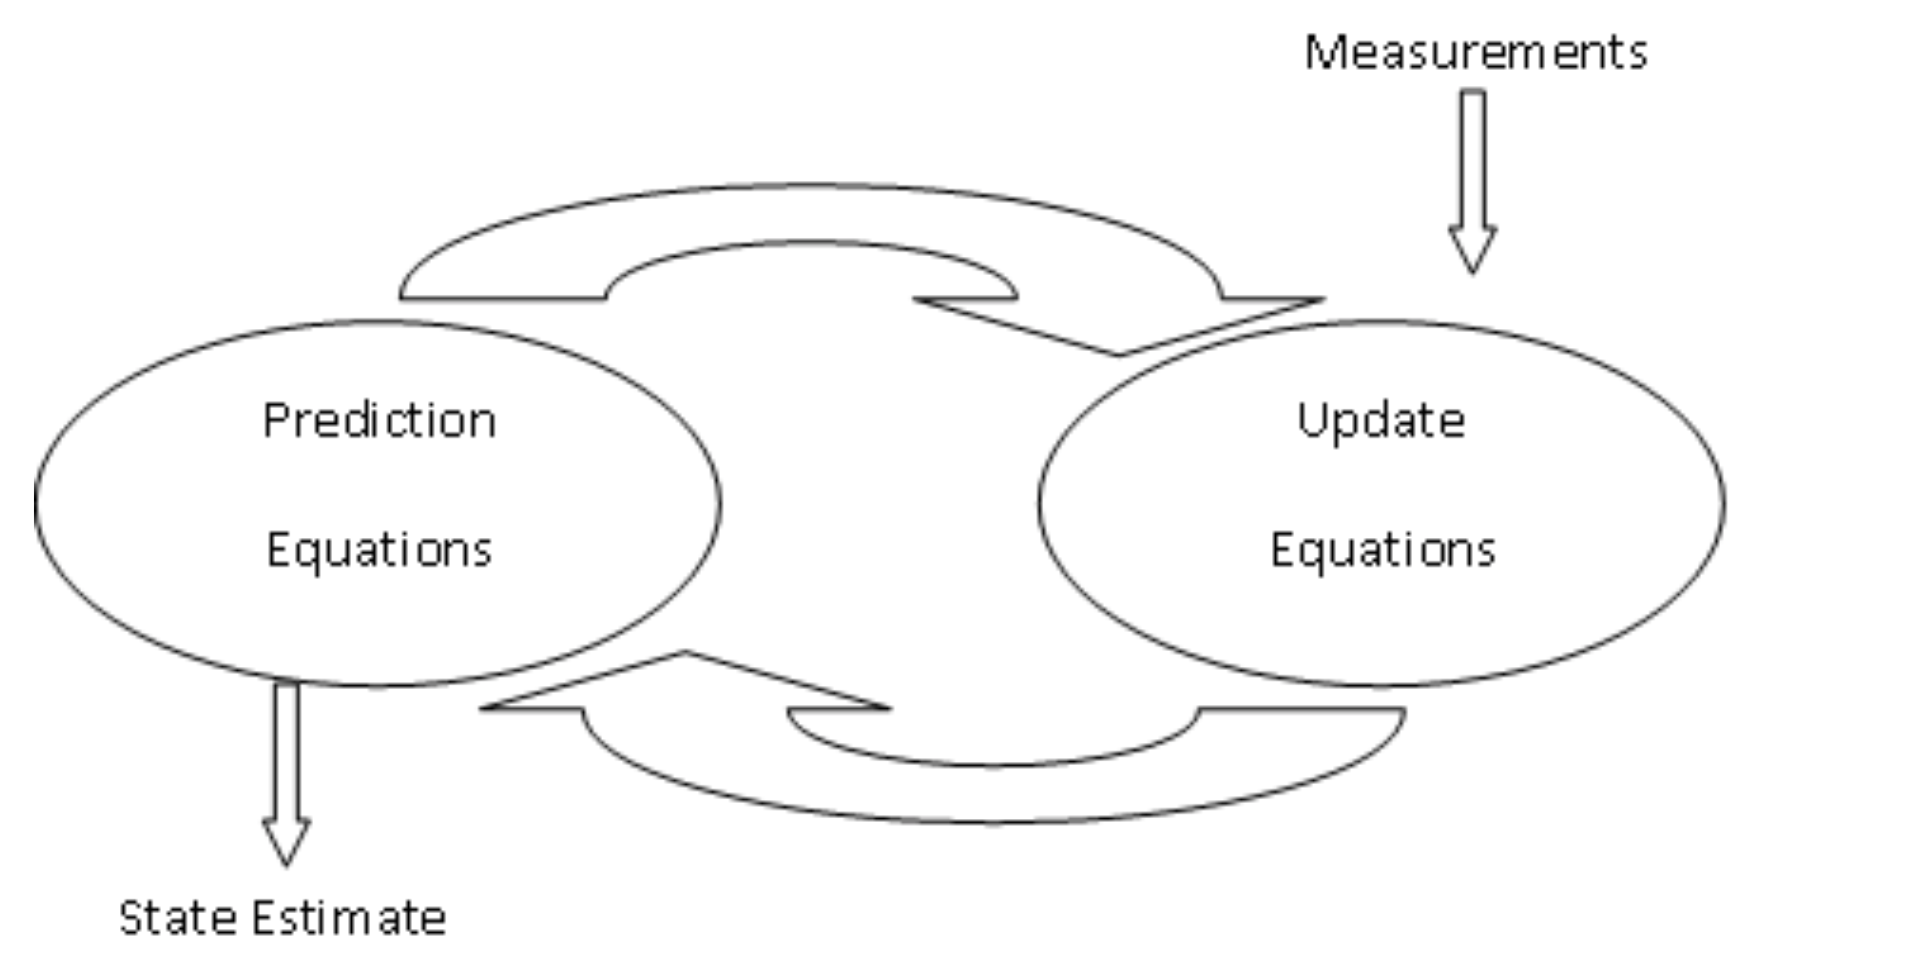
\includegraphics[scale = 0.3]{diagram.png}
    \caption{A basic diagram demonstrating the recursive nature of the Kalman Filter \cite{kohanbash_2014}.}
\end{figure}
\newpage


\begin{figure}[h]
    \centering
    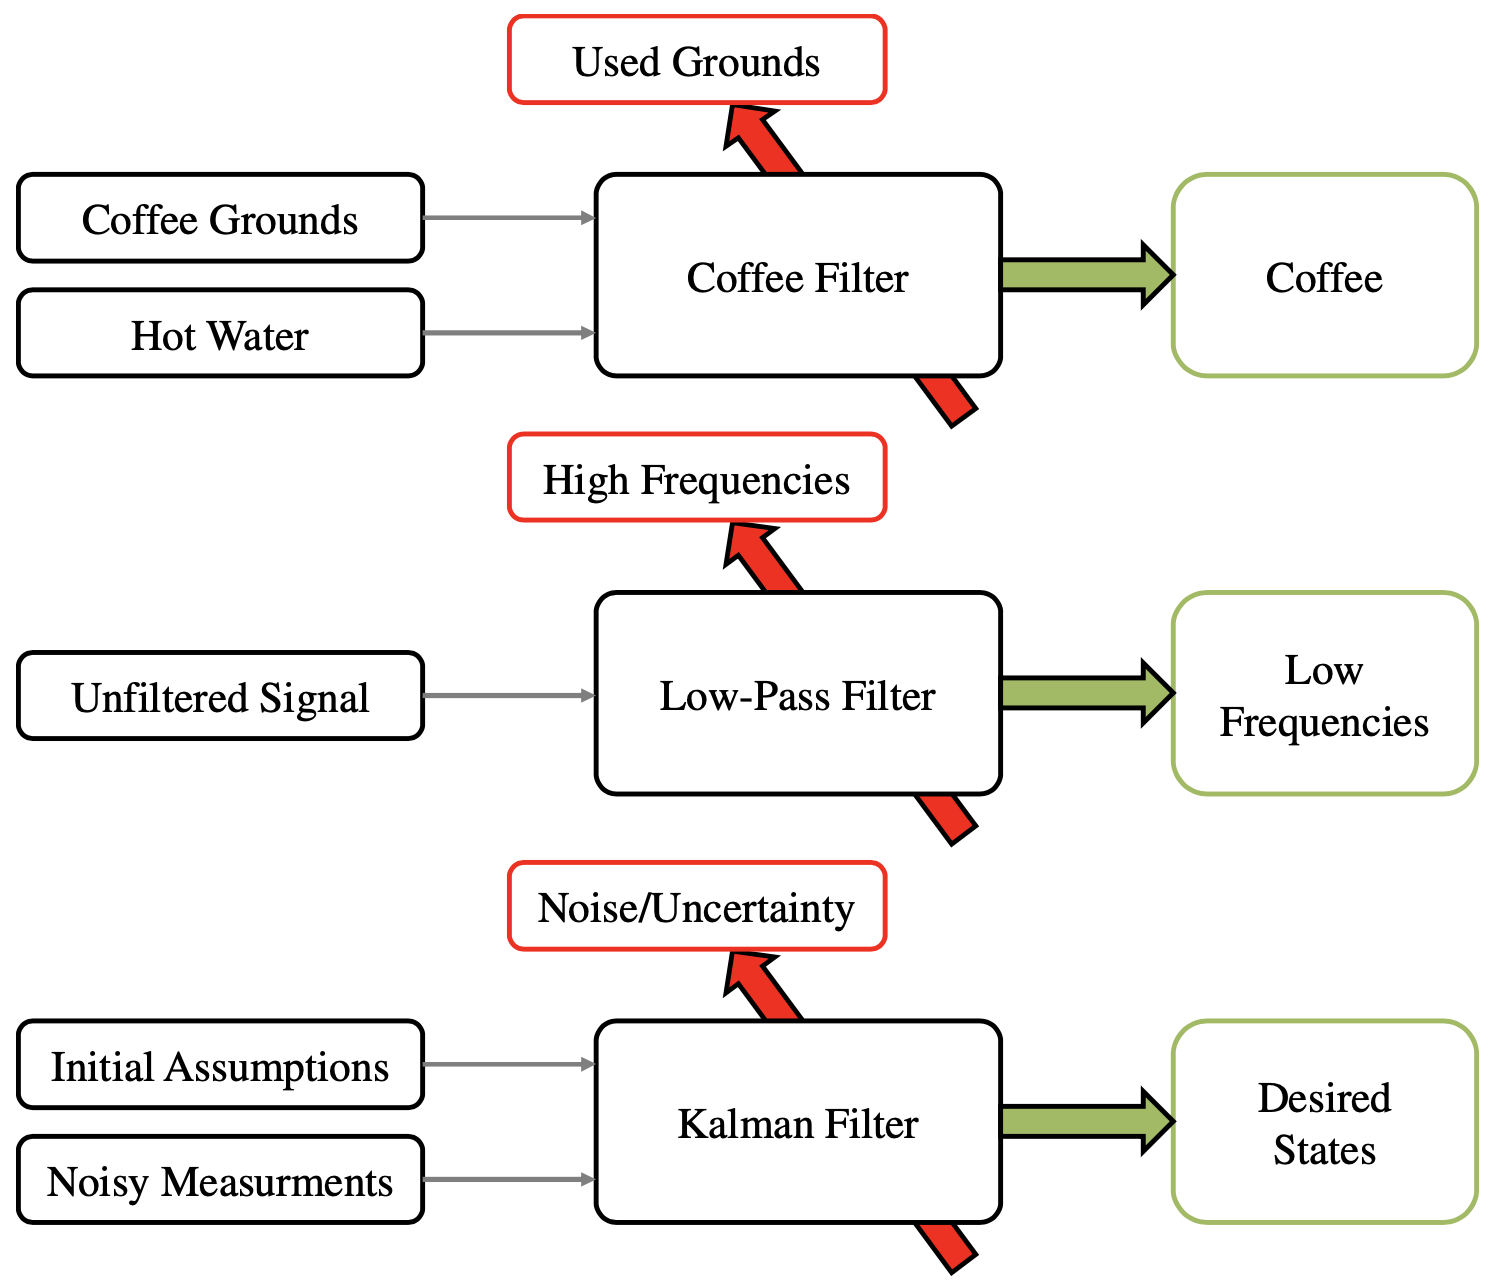
\includegraphics[scale = 0.4]{coffee.png}
    \caption{A simpler way to explore the KF is to facilitate a comparison with a coffee filter. This image is taken from a paper by Rhudy et al. comparing the Kalman Filter to a coffee filter \cite{article7}.}
    \end{figure}

\newpage

\noindent The most common application of KFs is in navigation, image processing, and finance. A relevant example is using computer vision to monitor and track vehicles in real time. This enables a traffic camera to know when to take a picture to capture a vehicle's license plate. Another example is the development of the Global Positioning Systems (GPS) \cite{lim_ong_lim_koo_2016}. The KF also has many aeronautical applications, which include long-distance flight and autopilot systems. In fact, the KF was initially created to help develop the navigation system in the Apollo Program \cite{kalmanbio}.  \\ \\


\noindent The Kalman Filter is named after its developer, Rudolph Emil Kalman. Kalman was born on May 19, 1930 in Budapest, Hungary. After arriving in the United States, Kalman completed his undergraduate studies and masters degree in electrical engineering from Massachusetts Institute of Technology and completed his doctoral degree in Columbia University. He would spend the next years of his life teaching. In the 1960s to 1970s he became a professor at Stanford university \cite{kalmanbio}. In the 1970s and 1990s, Kalman spent time as a professor of engineering at the University of Florida. Kalman is most known for his work on the Kalman Filter, which was developed in the late 1950s. The Kalman Filter greatly aided the United States' military projects, resulting in former President Obama to award Kalman the National Medal of Science in 2009. In addition, in 1985, Kalman was awarded the Kyoto Prize, which is the Japanese version of the Nobel Peace Prize. Kalman passed away July 2, 2016 at the age of 86 and is survived by his wife and two children \cite{Kalman_bio}. 

\newpage

\section{Kalman Filter Algorithm}

Before delving into the formal steps of the KF it is important to understand the underlying foundation of this algorithm. The goal of the Kalman Filter is to predict the new state of a system, after it undergoes some transformation. Let this be represented by 
\begin{align*}
	\frac{dx}{dt} = f(x) + \varepsilon ',
\end{align*}
where $\frac{dx}{dt}$ is the prediction of the states, $f$ is a linear function that transforms the states, given by $x$, and $ \varepsilon '$ is internal system noise. Since the system we are considering is linear, we can represent this transformation using matrix multiplication. Let matrix $M'$ be used to represent the transformation $f$ in order to approximate the equation above as
\begin{align*}
	\frac{dx}{dt} \approx M'x + \varepsilon '.
\end{align*}

\noindent The Kalman Filter works by generating predictions and making correction at various time steps. Let these time steps be denoted as $k$, such that $ k $ is a nonnegative integer and let $x_k$ be the estimate of the state variables at time $k$ with initial assumptions of the state variables beginning at $x_0$, such that $x_0 = \mathcal{N}(m_0, c_0)$, where $m_0$ and $c_0$ is mean and variance, respectively. 

\begin{figure}[h]
    \centering
    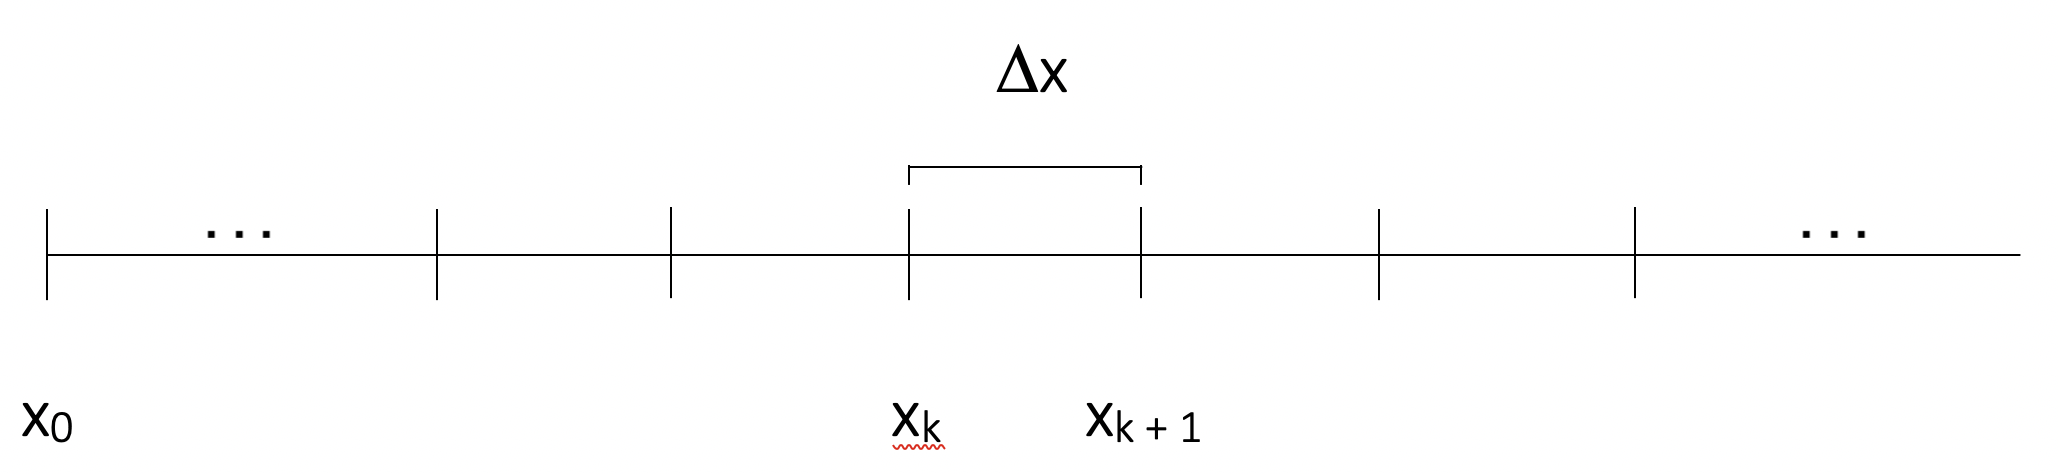
\includegraphics[scale = 0.3]{kgraph.png}
    \caption{A diagram showing discretized time steps of the system. Though this diagram depicts time steps that are equal, this should not be assumed for all cases.}
\end{figure}

\noindent Next, the system can be discretized by approximating $\frac{dx}{dt}$ using the limit definition of derivative:
\begin{align*}
	\frac{x_{k+1} - x_k}{\Delta t} &\approx M'x_k + \varepsilon '_k \\
	x_{k+1} - x_k &\approx M'x_k \Delta t + \varepsilon '_k  \Delta t \\
	x_{k+1} &\approx M'x_k \Delta t + \varepsilon '_k  \Delta t + x_k \\
	x_{k+1} &\approx (M' \Delta t + I)x_k + \varepsilon '_k  \Delta t.
\end{align*}


\noindent Next, substitute $M$ for $M' \Delta t + I$ and $\varepsilon_k$ for  $\varepsilon '_k  \Delta t $ to get the dynamics model:
\begin{align*}
	x_{k+1} \approx M x_k + \varepsilon_k,
\end{align*}
\noindent where $\varepsilon_k = \mathcal{N}(0, c_1)$ or Gaussian white noise. This general equation is significant to the generation of predictions and will continue to be used in different versions of the Kalman Filter. \\ 

\noindent Another important aspect of the KF is the incorporation of state measurements. It cannot be assumed that there will always be measurements for all states. More likely, there will only be measurements for a subset of states, Therefore, it is necessary to transform the prediction into a format that can be compared with state values. The transformed estimate of the system measurement at the next time step, call it $y_{k+1}$, is given by 
\begin{align*}
	y_{k+1} = H x_{k+1} + v_{k+1},
\end{align*}
where $H$ is the matrix observation function and $v_k$ is measurement noise vector at time step $k$ such that $v_k = \mathcal{N}(0, c_2)$ or Gaussian white noise. $H$, which can also be expressed as a matrix since the system is linear, enables the state variables to be linearly transformed to match the outputs of the system. The dimensions of $H$ reflects which state variables have measurable values in the system. It is not assumed that every state variable is measurable, so $H$ allows us to compare the measurable state variables to $x_k$. Simple applications of $H$ include creating matrices with 0's and 1's, with 1's denoting that a state variable is measurable and a 0's representing non-measurable states. In other cases, $H$ is an integer used as a scaling factor. \\ 

\noindent Given the dynamics model and data model, the algorithm of the KF can be discussed in greater depth. As a general overview, the KF algorithm consists of three major components:
\begin{enumerate}
  \item Initialize state variables
  \item Generate a prediction
  \item Update prediction with measurements from the system.
\end{enumerate}
The recursive component of the filter consists of repeating steps 2 and 3 repeatedly, while step 1 only needs to be done once. Details about each step are explored further below. \\

\begin{enumerate}
  \item Begin by initializing the state estimate and the initial state covariance matrix. The state estimate, $x_0$,  is a  column vector containing state variables, call them $x_a, x_b, \hdots, x_n$, such that $x_0= [x_a, x_b, \hdots, x_n]^T$, where $T$ is the transpose. The state estimate can be found by taking the expected value of the data, which is normally distributed. If the system states are finite, the expectation is denoted by
    \begin{align*}
        \mathbb{E}[x_0]   = \sum^n_{i = a} x_i p_i = [x_a p_a + x_b p_b + \hdots + x_n p_n]^T,
        %= \begin{bmatrix}
          % x_a \\
           %\vdots \\
           %x_ 
        % \end{bmatrix}.
    \end{align*}
    and if the system states are continuous case, the expectation is denoted by 
    \begin{align*}
        \mathbb{E}[x_0]   = \int^n_{a} xf(x)  dx
    \end{align*}
    
    
    where $f(x)$ is the probability density function. The state covariance matrix, $P_0$, is a square matrix whose contents are the covariance of the pairwise elements
    \footnote{Recall that the covariance of a variable with itself is the variance of the variable}.  A state covariance matrix is a symmetrical positive semi-definite square matrix whose diagonals correspond to the variance of a variable at location $i$ and elsewhere is the covariance of the pairwise elements. In practice, covariance matrices help us better understand the spread of data. For the case of the KF, calculating the state covariance is necessary for computing Kalman Gain, which is used in the correction step. Calculating the state covariance matrix can be done by 
    \begin{align*}
      P_0 =
      \begin{bmatrix}
           var(x_a)  & \hdots & cov(x_a,x_n) \\
           \vdots & \ddots & \vdots \\
           cov(x_n, x_a)  & \hdots & var(x_n )
         \end{bmatrix} .
  \end{align*}
  Enough should be known about the modeled system to generate these values. In the case where one knows the true value of the initial states, the state covariance would have all 0 values. On the other hand, if one is unsure of the initial values, values in $P_0$ are expected to be higher. It is important to initialize the model with values close to the true value, else the system will converge at a slow rate.  \\ 
  
 \item After initializing the state estimate and state covariance, a prediction can be generated. The estimate of the system at the next time step, $x_{k+1}$,  is given by
  \begin{align*}
      x_{k|k-1} = F x_{k-1|k-1} + w_{k-1} ,
  \end{align*} 
  where $F$ is the state transition matrix and $w_k$ is the process noise vector. Every state variable contained in $x_k$ is defined by a linear differential equation. These linear differential equations can be used to generate the F matrix. Therefore, F should be a square matrix whose dimension is equal to the number of states variables. \\ \\
  $w_k$ is the process noise vector at time k. Process noise can be thought of as the model's accuracy. When process noise is 0, it implies that the model is perfectly accurate and does not have to correct for incoming system measurements. On the other hand, high process noise will essentially restart the system based on incoming measurements. $w_k$ has the same dimensions as $x_k$, allowing us to identify whether or not to adjust the equations for the state variables. \\
  
  \item Next, correct the prediction with incoming measurements from the system. Begin by calculating the state covariance matrix in order to calculate Kalman Gain. The state covariance matrix at time step $k$ given the last time step, is 
    \begin{align*} 
        P_{k | k -1} = F P_{k - 1} F^T + Q_{k-1}, 
    \end{align*}
    where $F^T$ is the transpose of $F$, and $Q_{k}$ is the process noise covariance of $w_k$.
    The Kalman Gain at time step $k$, is given by
    \begin{align*} 
        K_k = P_{k | k - 1} H^T (H P_{k | k - 1} H^T + R_k)^{-1},
    \end{align*}
      where $H^T$ is the transpose of the observation matrix and $R$ is the measurement noise covariance matrix. \\ 

     \noindent From this equation, one can see that balancing $Q$ and $R$ is critical for model performance. Larger values of $Q$ indicate higher modeling error, which leads to a higher Kalman Gain and increased model correction. On the other hand, large values of $R$ imply high measurement error, leading to a lower Kalman Gain and less model correction. \\ 
     
     \noindent The Kalman Gain is a measure of how much to change the model based on incoming data. Low values of the Kalman Gain imply the model is accurate while higher values indicate the model should adjust based on the incoming data.  \\ 
   
     Next, calculate the transformed prediction in order to correct the prediction. The transformed state vector, $\hat y_k$, is given by
    \begin{align*}
        \hat y_k = H x_{k|k-1} + v_k,
    \end{align*}
    
    where $v_k$ is measurement noise, which is added to account for measurement error.
    The corrected prediction, $ x_{k|k-1} $, is given by
    \begin{align*} 
        x_{k|k} = x_{k|k - 1} + K_k(y_k - \hat y_{k}),
    \end{align*}
   where  $y_k$ is the actual measurements of the system, $K_k$ is the Kalman Gain matrix at time step $k$, and $x_{k-1}$ are the values of the state variable at the last time step. The quantity $y_k - \hat y_{k}$ is also known as measurement residual or innovation.  Later on, we will see how this value is used to gauge model performance. \\
   
      The final step is to update the state covariance matrix, $P_k $, through the equation
    \begin{align*} 
        P_{k|k} = (I - K_k H) P_{k | k-1},
    \end{align*}
    where $I$ is the identity matrix, $K_k$ is the Kalman Gain at time step $k$, $H$ is the observation matrix, and $P_{k|k-1}$ is the state covariance at time step $k$ given the last time step. $ P_k $ will be used in the next iteration of the filter. \\ \\
\noindent Steps 2 and 3 may be repeated to progressively generate more accurate predictions.
\end{enumerate} 


\newpage

\begin{center}
\begin{table}
\centering
\caption{Description of all variables in the Kalman Filter} \label{tab:sometab}
\begin{tabular}{ |p{2cm}||p{5cm}|p{2cm}| }
    \hline
    \multicolumn{3}{|c|}{Variables in the Kalman Filter } \\ 
    \hline
    Variable & Description & Dimensions \\
    \hline
    $x$ & State variables  & $x \times 1$ \\
    $\hat y$ & Transformed state vector  & $y \times 1$ \\
    $y$ & Actual system measurement(s) & $y \times 1$ \\
    $v$ & Measurement noise vector & $y \times 1$\\
    $w$ & Process noise vector & $x \times 1$\\
    $F$ & State function  & $x \times x $  \\ 
    $H$ & Observation function & $y \times x$\\
    $K$ & Kalman Gain  & $x \times y$\\
    $Q$ & Process noise covariance  & $x \times x$ \\
    $R$ & Measurement noise covariance &  $y \times y$\\
    $P$ & Covariance matrix & $x \times x $  \\ 
    \hline
\end{tabular}
\end{table}
\end{center} 

\newpage

% \section{Assessing Model Performance}



